\chapter{Design}

\begin{flushleft}
In this chapter, I describe the design of the Android application for gathering the data as well as the sever side implementation to store and compute the information. 
First, I will start with a brief description of the two components and will follow with my design decisions and my reasons for the choices. 
\end{flushleft}

\section{Functionality Overview}
The purpose of the software is to gather information from a mobile device of a participant while he/she is working on a programming task. Afterwards the application sends the collected data to a server for further processing and analysis. The participant also simultaneously submits the written code which code quality will be detected and then correlated with the processed mobile device information. 


\section{Mobile Application Design}

% Define bar chart colors
%
\definecolor{others}{HTML}{e78d1c}
\definecolor{android}{HTML}{a4c639}
\definecolor{ios}{HTML}{1c90e7}

\begin{figure}
	\centering
	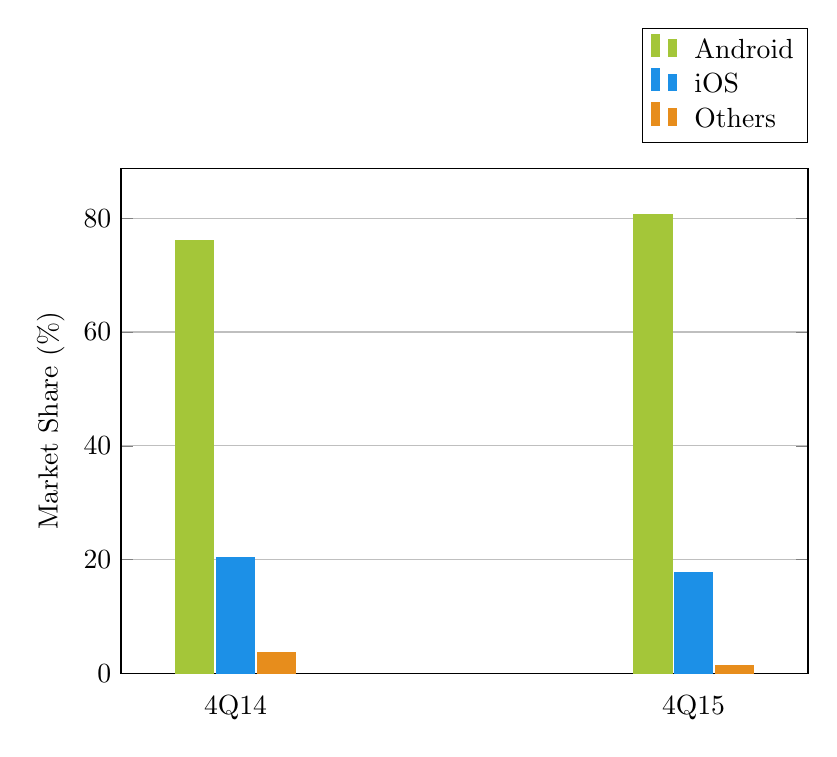
\begin{tikzpicture}
        \begin{axis}[
            width  = 0.85*\textwidth,
        	height = 8cm,
        	major x tick style = transparent,
        	ybar=2*\pgflinewidth,
        	bar width=14pt,
        	ymajorgrids = true,
        	ylabel = {Market Share (\%)},
        	symbolic x coords={4Q14, 4Q15},
       	 	xtick = data,
        	scaled y ticks = false,
        	enlarge x limits=0.25,
        	ymin=0,
        	legend cell align=left,
        	legend style={
                at={(1,1.05)},
                anchor=south east,
                column sep=1ex
        	}
      	]
     	\addplot[style={android,fill=android,mark=none}]
            coordinates {(4Q14, 76.0) (4Q15, 80.7)};

        \addplot[style={ios,fill=ios,mark=none}]
             coordinates {(4Q14, 20.4) (4Q15, 17.7)};

        \addplot[style={others,fill=others,mark=none}]
             coordinates {(4Q14, 3.7) (4Q15, 1.5)};

        \legend{Android, iOS, Others}

        \end{axis}
 	\end{tikzpicture}
 	\caption{Smartphone OS marketshare}\label{result}
 	\vspace{10 mm}
\end{figure}

\begin{flushleft}
In quarter 4 of 2015 Android had a market share of 80.7\% in smart-phone sales by operating system (see Figure \ref{result}). The trend also shows that the number increased from the last year \cite{gartnerMobileOSMarketshare}. Therefore I decided to realize the mobile application implementation for Android in order to be able to work with more users who have access to that application.
An alternative to the native implementation (e.g. iOS or Android) could have been a hybrid application. A hybrid apps is based on web-technology and using the addvantage of resposive web design to be able to work with every aspect ratio and resolution on an mobile device. One way doing that would be by using a framework such as PhoneGap, wich internally creates a native webview applicationand just loads the hybrid JavaScript, HMTL, CSS in it. Another software for cerating a hybrid solution is Titanum accelerator which itself is using native UI components. Both frameworks have the advantage is the simple development and the OS independence. The problem with hybrid apps are the performance and limited accessiblity to hardware components including some sensors \cite{holzinger2012making}.  

The Android application make use of its build in sensors and information provided by the Android operating system. Different than iOS, Android is an OS that can be installed of different devices from different vendors and with different hardware components \cite{goadrich2011smart}. Thus the buit in sensors which are clustered in motion sensors, environmental sensors and position sensors \cite{androidDevelopers} can differ between the different devices. Components which are required for standard functionality such as making phone calls are more common than other sensors. For example the the microphone for recording the users voice or the light sensor, which is used to detect whether the user has the phone at his ear can be found in almost every mobile android device. 


\end{flushleft}

\section{Server Backend Design}


Zhu, Hengshu, et al. \cite{zhu2015mining} read the device logs and get all the logged device more information about the apps being used etc.
Sandboxing is an Android security concept that only allows an app to access the data of the app itself and isolates the content for other applications. Thus it is impossible to access the device logs via an app without having physical access to the device. 
In terms of the ideas for future usage of the app 



